\documentclass[t]{beamer}

\usepackage[ngerman]{babel}
\usepackage[utf8]{inputenc}
\usepackage{amssymb}
\usepackage{amsmath}
\usepackage{amsthm}
\usepackage{amsfonts}
\usepackage{setspace}
\usepackage{tikz}
\usepackage{lmodern}

\usetheme{Madrid}
\usecolortheme{default}
\date{\today}

\title{Simulating Visual Geometry}
\author{Patrick Bayer}
\linespread{1.5}

\begin{document}
	\begin{frame}{Die Simulationsmethode}
	\textcolor{blue}{Shape Matching:}
	\begin{itemize}
		\item Simulation von Elastizität
		\item Arbeitet mit Partikeln ohne Verbindungen
	\end{itemize}
	\begin{center}
		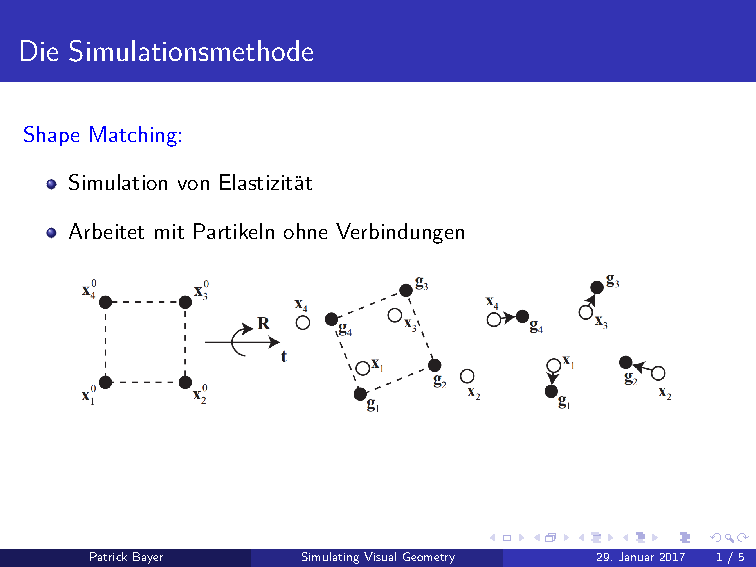
\includegraphics[scale = 0.25]{ShapeMatching.png}
	\end{center}
	
\end{frame}


\begin{frame}{Die Simulationsmethode}
	\begin{itemize}
		\item Berechne $\mathbf{R}, \mathbf{\bar{t}}$ und $ \mathbf{t}$ durch Minimieren von \\
		\begin{center}
			$\sum\limits_{\mathnormal{i}}\mathnormal{\mathbf{m}_i}($\textbf{R}$(\mathnormal{\mathbf{\bar{x}}_i}-\mathnormal{\mathbf{\bar{t}}})+$\textbf{t}$-\mathnormal{\mathbf{x}_i})^2$
		\end{center}
		\item Es stellt sich heraus, dass \\
		\begin{center}
			$\mathnormal{\mathbf{\bar{t}}}=\mathnormal{\mathbf{\bar{x}}_{cm}}=\frac{\sum_{\mathnormal{i}}\mathnormal{\mathbf{m}_i} \mathnormal{\mathbf{\bar{x}}_i}}{\sum_{\mathnormal{i}}\mathnormal{\mathbf{m}_i}}$ and \textbf{t} $=\mathnormal{\mathbf{x}_{cm}}=\frac{\sum_{\mathnormal{i}}\mathnormal{\mathbf{m}_i \mathbf{x}_i}}{\sum_{\mathnormal{i}}\mathnormal{\mathbf{m}_i}}$
		\end{center}
		\item Seien $\mathnormal{\mathbf{q}_i}=\mathnormal{\mathbf{\bar{x}}_i}-\mathnormal{\mathbf{\bar{x}}_{cm}}$ und
		$\mathnormal{\mathbf{p}_i}=\mathnormal{\mathbf{x}_i}-\mathnormal{\mathbf{x}_{cm}}$, dann minimiere \\
		\begin{center}
			$\sum\limits_{\mathnormal{i}}\mathnormal{\mathbf{m}_i}(\mathnormal{\mathbf{A}\mathbf{q}_i}-\mathnormal{\mathbf{p}_i})^2$
		\end{center}
		wobei \textbf{A} die optimale lineare Transformation ist.	
		
	\end{itemize}
\end{frame}

\begin{frame}{Die Simulationsmethode}
	\begin{itemize}
		\item Es stellt sich heraus, dass
		\begin{center}
			\textbf{A} $=(\sum\limits_{\mathnormal{i}}\mathnormal{\mathbf{m}_i}\mathnormal{\mathbf{p}_i}\mathnormal{\mathbf{q}_i^T})(\sum\limits_{i}\mathnormal{\mathbf{m}_i}\mathnormal{\mathbf{q}_i}\mathnormal{\mathbf{q}_i^T})^{-1}=\mathnormal{\mathbf{A}}_{pq}\mathnormal{\mathbf{A}}_{qq}$
		\end{center}
		\item $\mathnormal{\mathbf{A}}_{qq}$ ist symmetrisch, enthält also keine Rotation
		\item Eine Polarzerlegung von $\mathnormal{\mathbf{A}}_{pq}$ liefert \\
		\begin{center}
			$\mathnormal{\mathbf{A}_{pq}}=$ \textbf{RS} wobei \textbf{S} $=\sqrt{\mathnormal{\mathbf{A}_{pq}^T} \mathnormal{\mathbf{A}_{pq}}}$ und \textbf{R} $=\mathnormal{\mathbf{A}_{pq}}\mathnormal{\mathbf{S^{-1}}}$
		\end{center}
		\item Berechne die Zielposition jedes Partikels
		\begin{center}
			$\mathnormal{\mathbf{g}_i}=\mathnormal{\mathbf{R}}(\mathnormal{\mathbf{\bar{x}}_i}-\mathnormal{\mathbf{\bar{x}}_{cm}})+\mathnormal{\mathbf{x}_{cm}}$ 
		\end{center}
	\end{itemize}
\end{frame}

\begin{frame}{Die Simulationsmethode}
	\begin{itemize}
		\item Co-Planarität oder Co-Linearität der Punkte $\Rightarrow$ Unstabilität
		\item $\mathnormal{\mathbf{A}}_{pq}$ für zwei Partikelmengen mit Moment Matrizen $\mathnormal{\mathbf{A}_1}$ und $\mathnormal{\mathbf{A}_2}$ 
		\begin{center}
			$\mathnormal{\mathbf{A}}_{pq}=\sum\limits_{i}\mathnormal{\mathbf{m}_i \mathbf{x}_i \mathbf{\bar{x}}^T_i}-M\mathnormal{\mathbf{x}_{cm} \mathbf{\bar{x}}_{cm}^T}$
		\end{center}
		\item $\mathnormal{\mathbf{A}}_{pq}$ mit Moment Matrizen $\mathnormal{\mathbf{A}_i}$ für jedes einzelne Partikel
		\begin{center}
			$\mathnormal{\mathbf{A}_{pq}}=\sum\limits_{i}(\mathnormal{\mathbf{A}_i}+\mathnormal{\mathbf{m}_i \mathbf{x}_i \mathbf{\bar{x}}_i^T})-M\mathnormal{\mathbf{x}_{cm} \mathbf{\bar{x}}_{cm}^T}$
		\end{center}
		wobei $\mathnormal{M}$ die Summe der Massen $\mathbf{m}_i$ ist
	\end{itemize}
\end{frame}

\begin{frame}{Die Simulationsmethode}
	\begin{itemize}
		\item Berechne die Moment Matrizen der einzelnen Partikel mit orthonormaler Orientierungsmatrix \textbf{R} für Kugeln mit Radius $r$ Volumen $V_r$ und Ellipsoide mit Radien $\mathnormal{a, b}$ und $\mathnormal{c}$ 
		\begin{center}
			$\mathnormal{\mathbf{A}_{sphere}}= \int_{V_r}\rho(\mathbf{Rx})\mathbf{x}^T dV = \frac{1}{5}mr^2\mathbf{R}$
		\end{center}
		\begin{center}	
			$\mathnormal{\mathbf{A}_{ellipsoid}}= \frac{1}{5}m
			\begin{bmatrix}
			a^2& 0& 0 \\
			0& b^2& 0 \\
			0& 0& c^2
			\end{bmatrix}\mathbf{R}$
		\end{center}
	\end{itemize}
\end{frame}
\end{document}